\section{Скалярное поле}

\subsection{Определение}

	\begin{definition}
	Если в каждой точке пространства задана скалярная функция \( u = u(x, y, z) \), то говорят, что в пространстве определено скалярное поле \( u = u(x, y, z) \). При этом предполагается, что функция \( u \) принимает конечные действительные значения.
	\end{definition}
	
	Примеры скалярных полей:
	\begin{itemize}
	\item \( T = T(x, y, z) \) -- поле распределения температур;
	\item \( P = P(x, y, z) \) -- поле давления;
	\item \( \rho = \rho(x, y, z) \) -- поле распределения плотности;
	\item \( \varphi = \varphi(x, y, z) \) -- поле потенциала.
	\end{itemize}
	
	Если \( u = u(x, y, z, t) \), то поле называется нестационарным.

\subsection{Поверхности и линии уровня скалярного поля}

    Геометрическим представлением скалярного поля являются поверхности уровня.

    \begin{definition}
        Поверхность уровня скалярного поля \( u(x,y,z) \) -- это геометрическое место точек в пространстве, для которых выполняется равенство \( u(x,y,z) = \const = C \).
    \end{definition}

    \begin{figure}[h]
        \center
        \begin{minipage}[h]{0.49\textwidth}
        \center{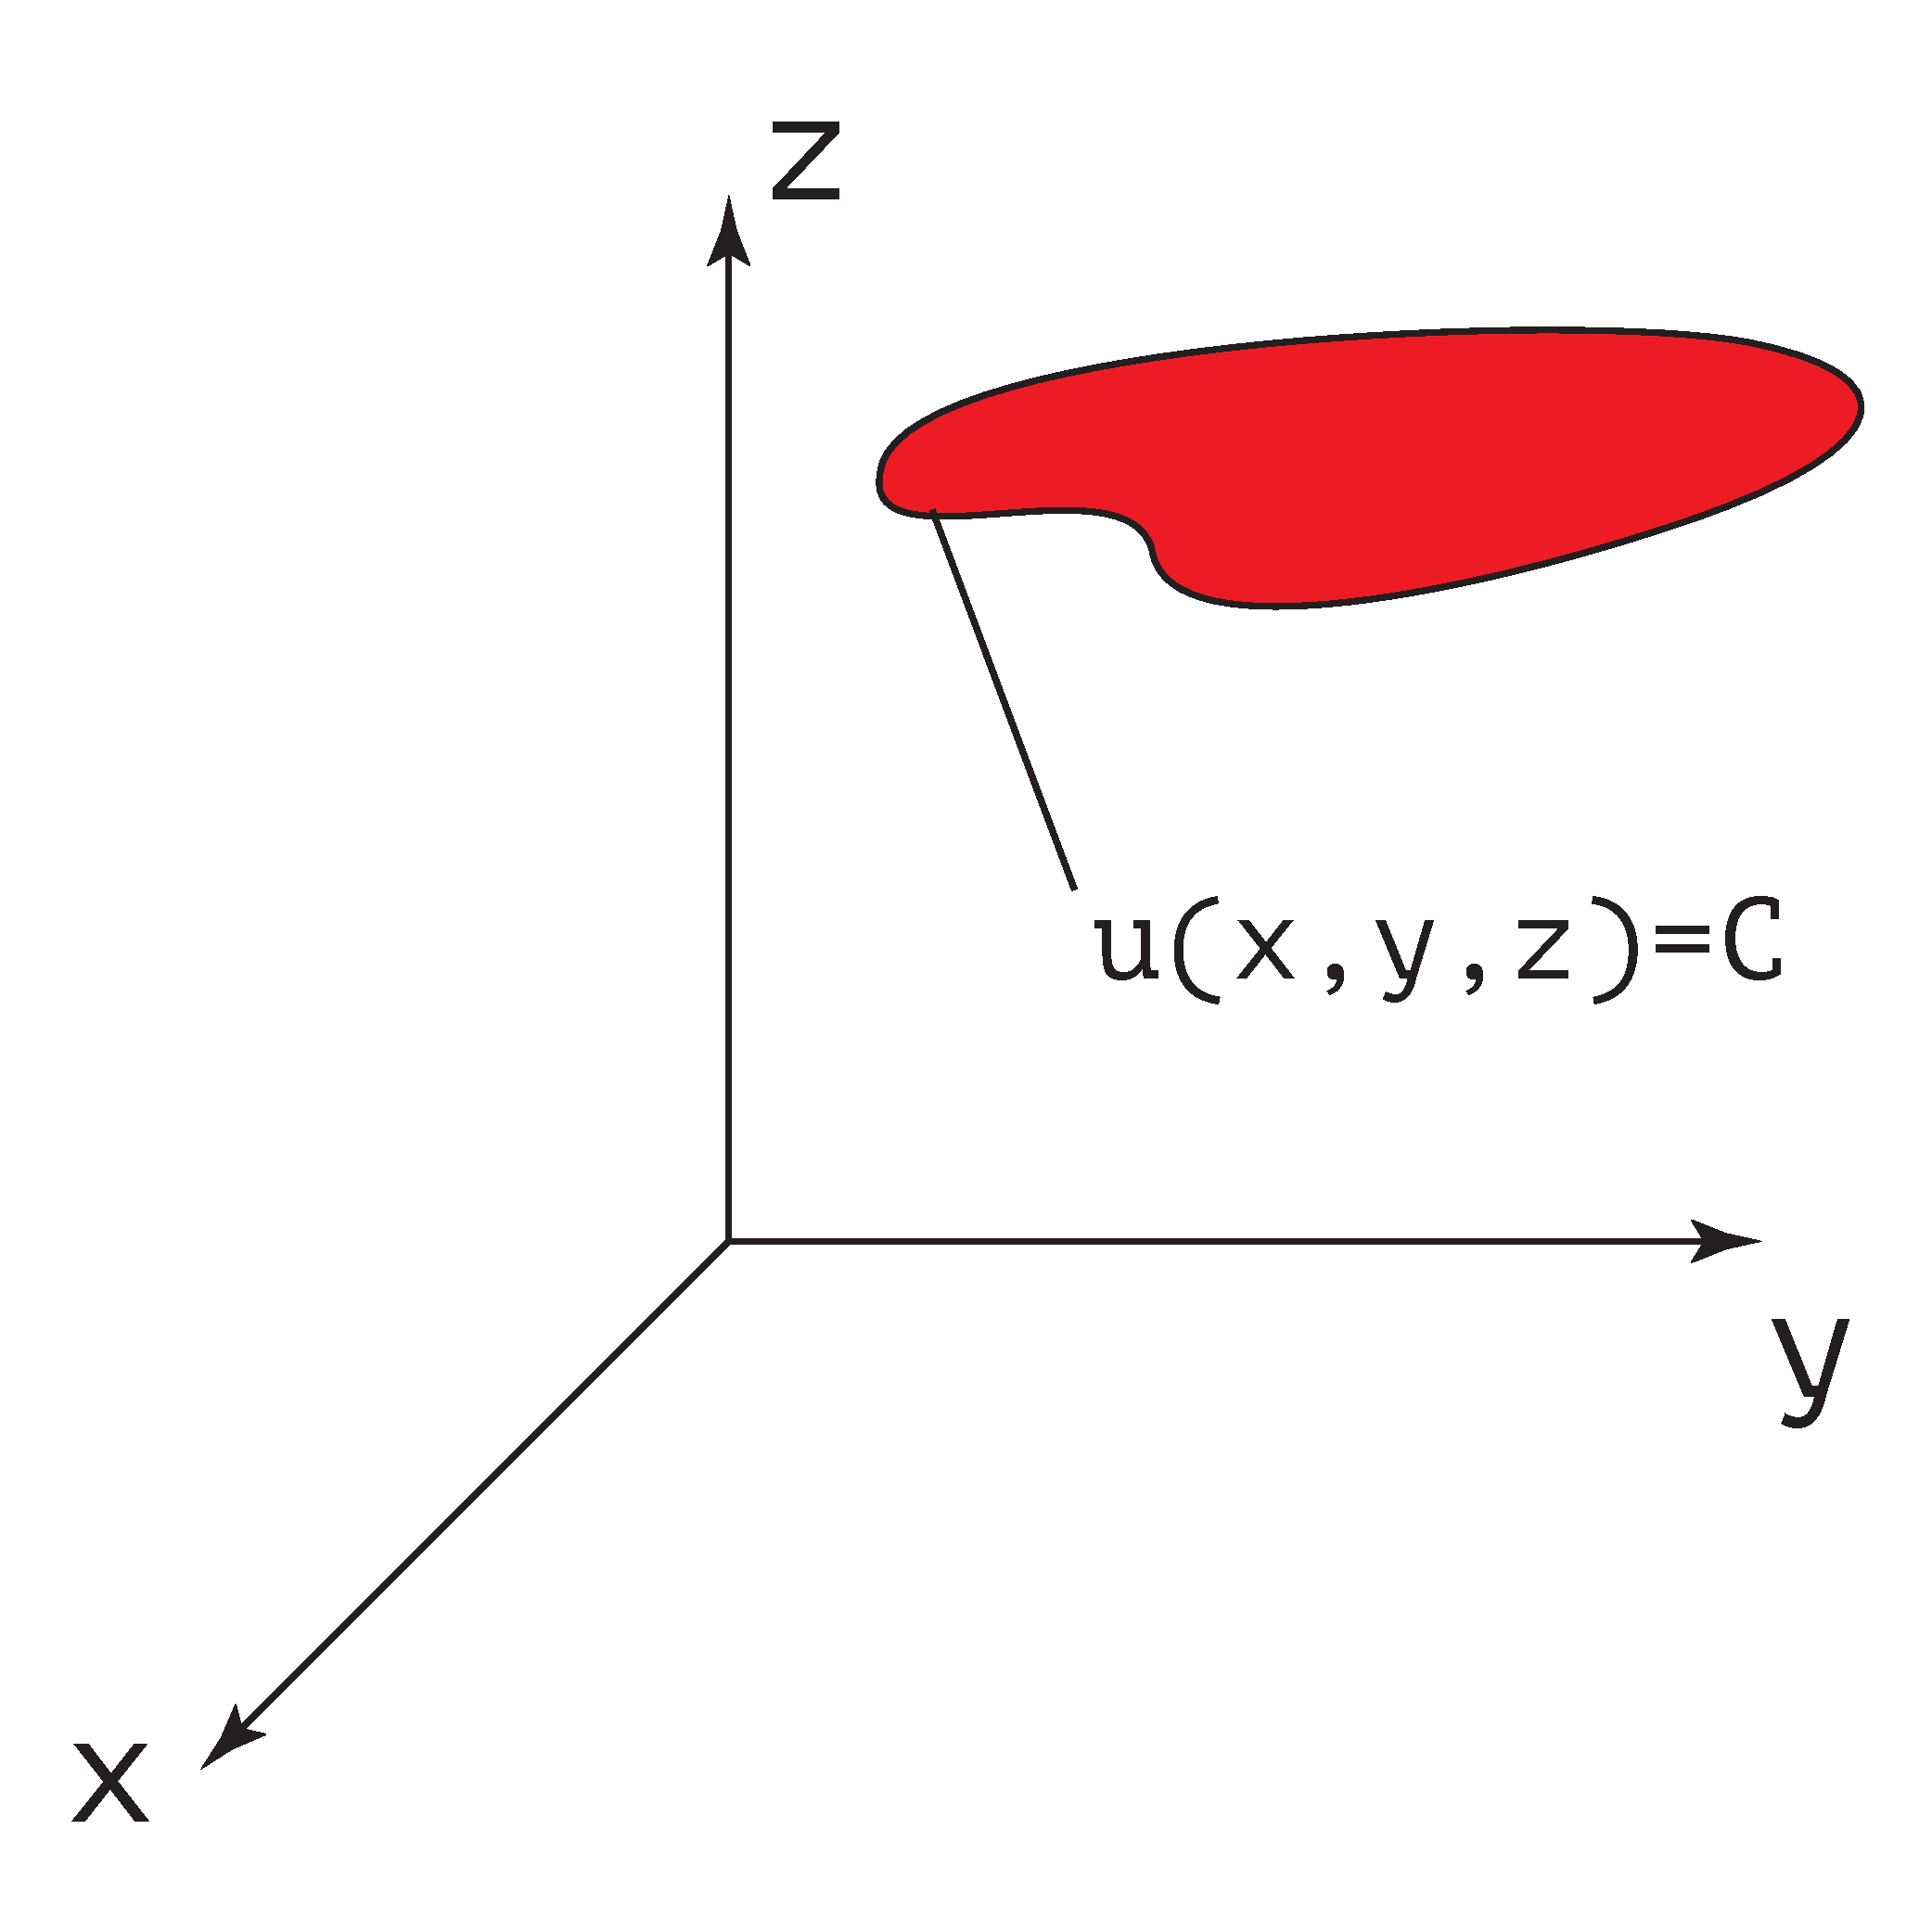
\includegraphics[width=0.47\textwidth]{lec02/surface_of_level.pdf} \\ Поверхность уровня}
        \end{minipage}
        \hfill
        \begin{minipage}[h]{0.49\textwidth}
        \center{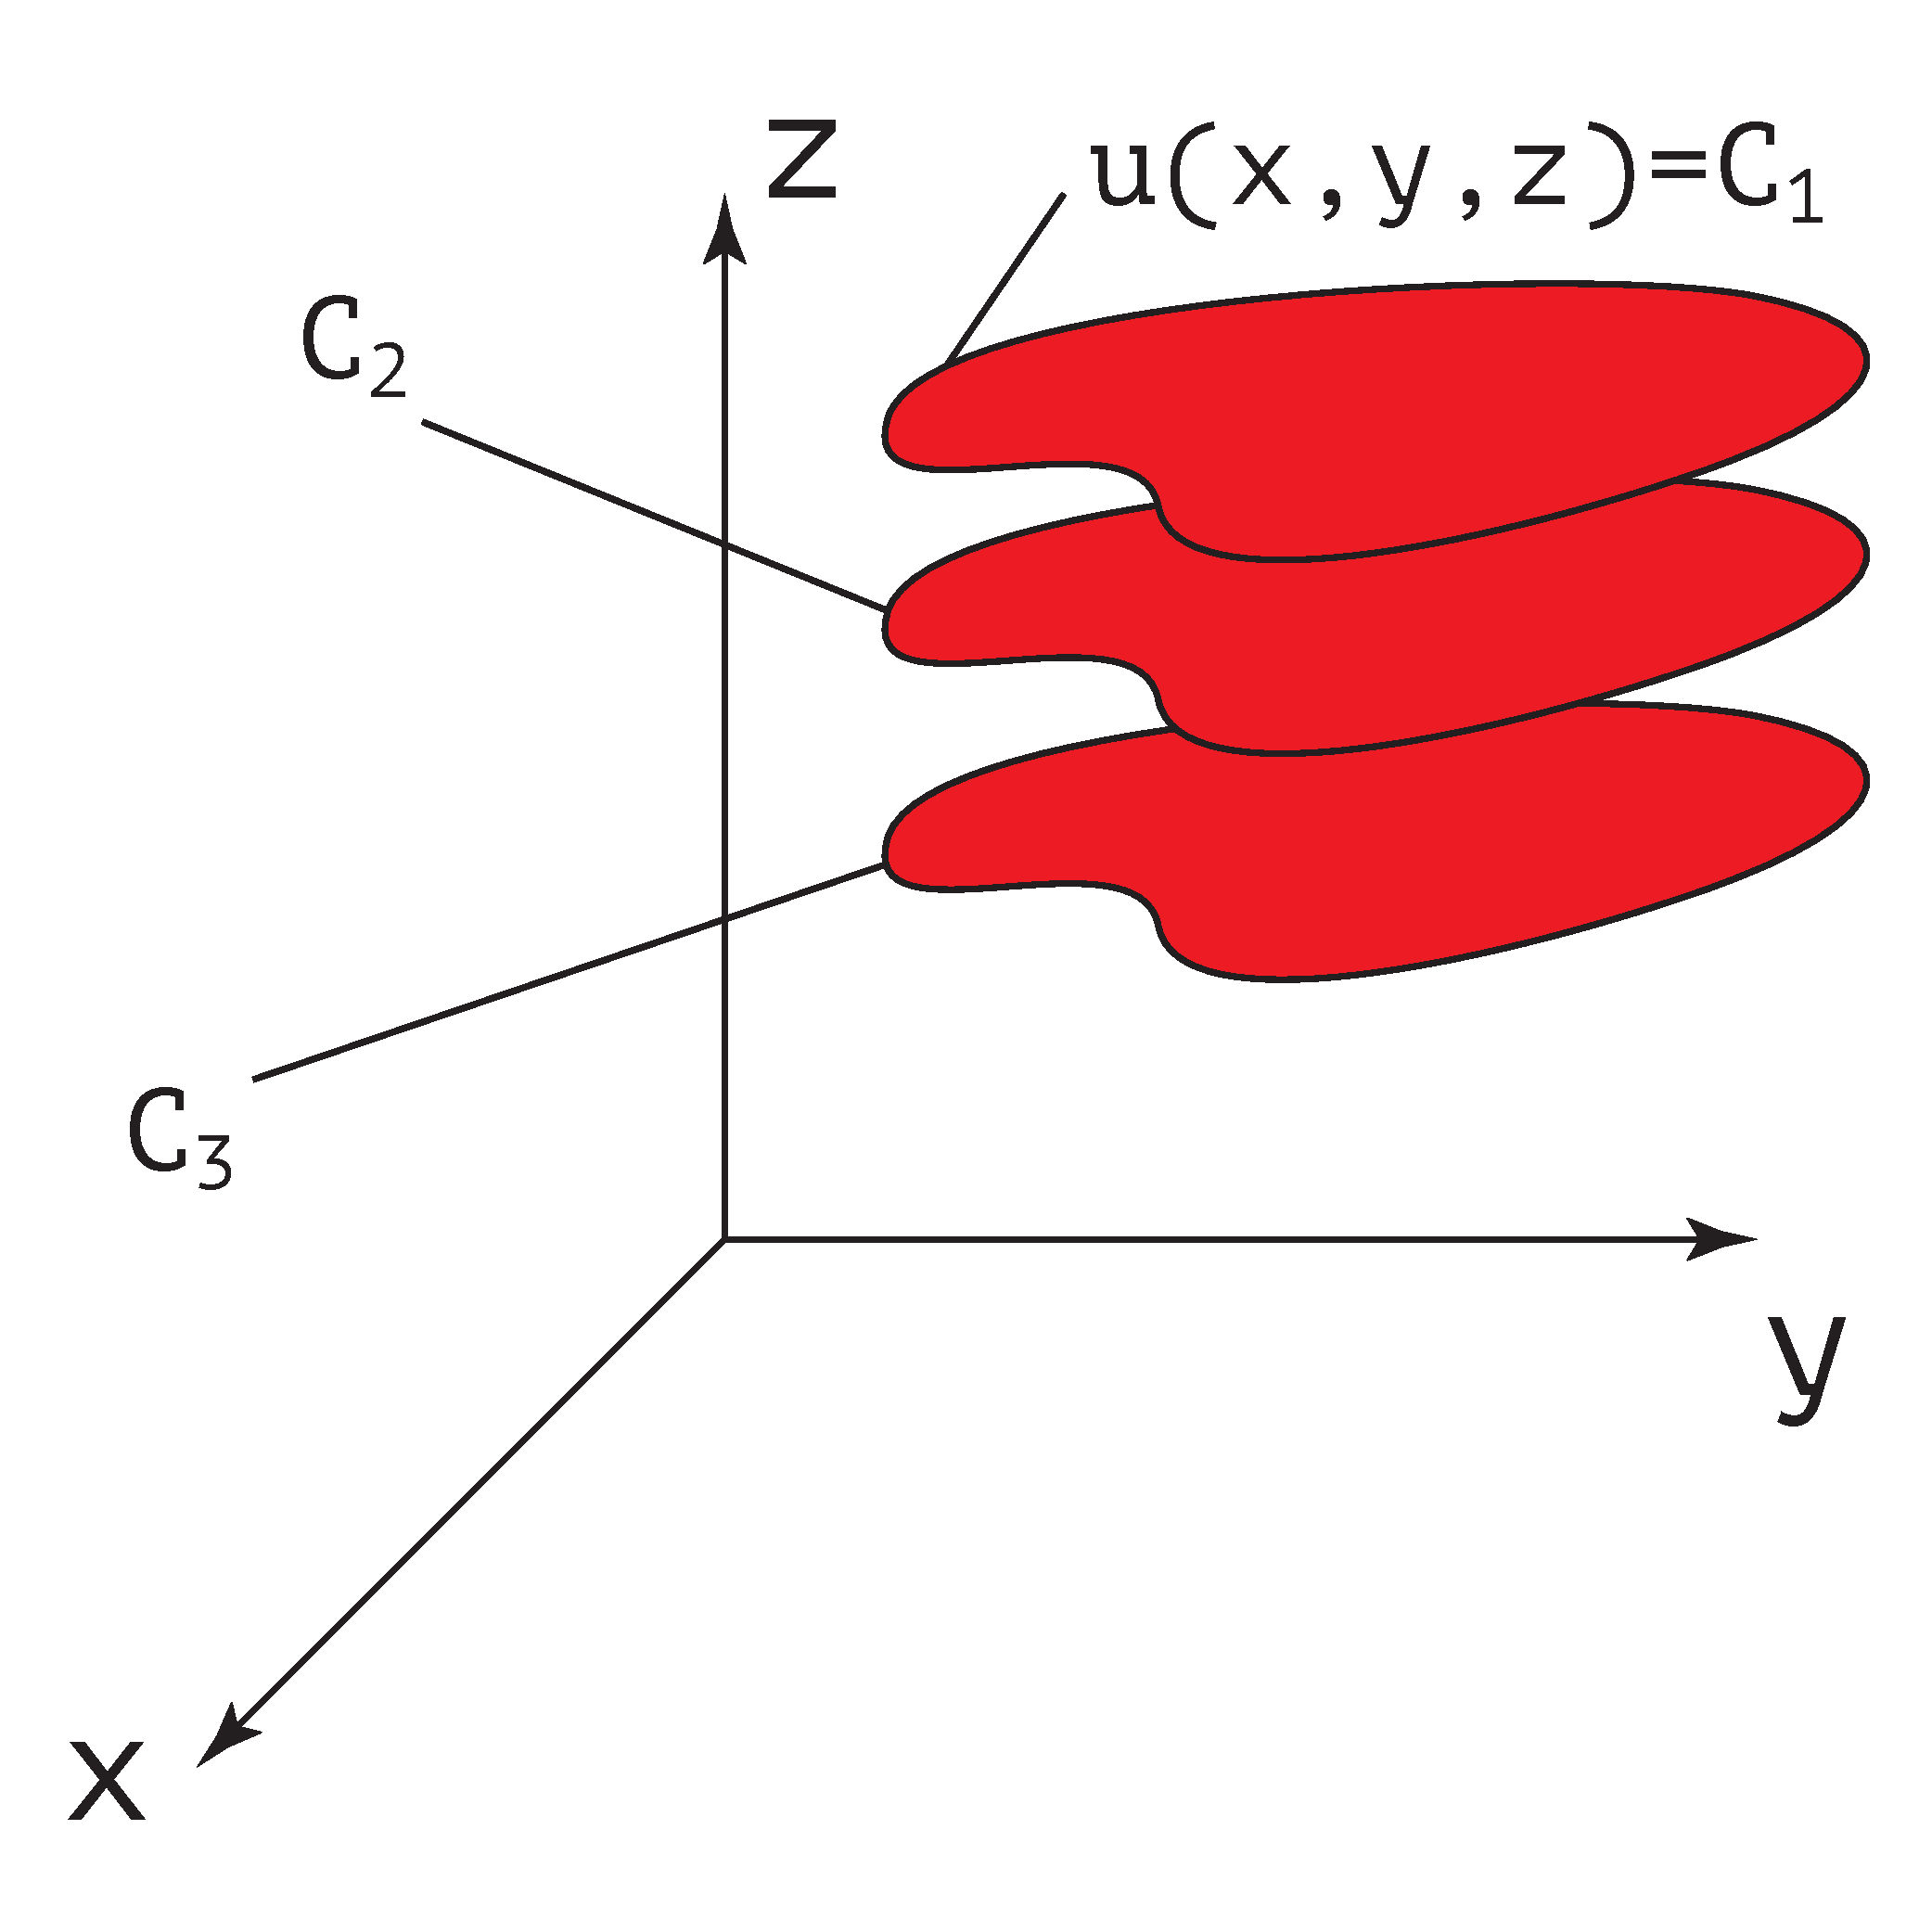
\includegraphics[width=0.47\textwidth]{lec02/family_of_surfaces.pdf} \\ Семейство поверхностей уровня}
        \end{minipage}
        \end{figure}

    \begin{remark}
        Так как \( u(x,y,z) \) по определению однозначна, то поверхности уровня не пересекаются.
    \end{remark}

    \begin{example}
        Поверхностями уровня потенциала точечного заряда являются концентрические сферы.
    \end{example}

    \begin{example}
        Семейством эквитемпературных поверхностей тонкой нагретой нити является система коаксиальных цилиндров.
    \end{example}

    \begin{example}
        Определить поверхности уровня скалярного поля \( u = \vec{a}\cdot\vec{r} \), где \( \vec{a} \) -- постоянный вектор.
    \end{example}

    \begin{solution}
    
    \[ u = a_xx + a_yy + a_zz = C_n. \]
    Это уравнение задаёт семейство плоскостей.
    \end{solution}

    \begin{remark}
        Если функция \( u = u(x,y) \), то поле называется плоским или двумерным, и его геометрическим представлением являются линии уровня на плоскости xOy.
    \end{remark}

    \begin{figure}[h]
        \center
        \begin{minipage}[h]{0.49\textwidth}
        \center{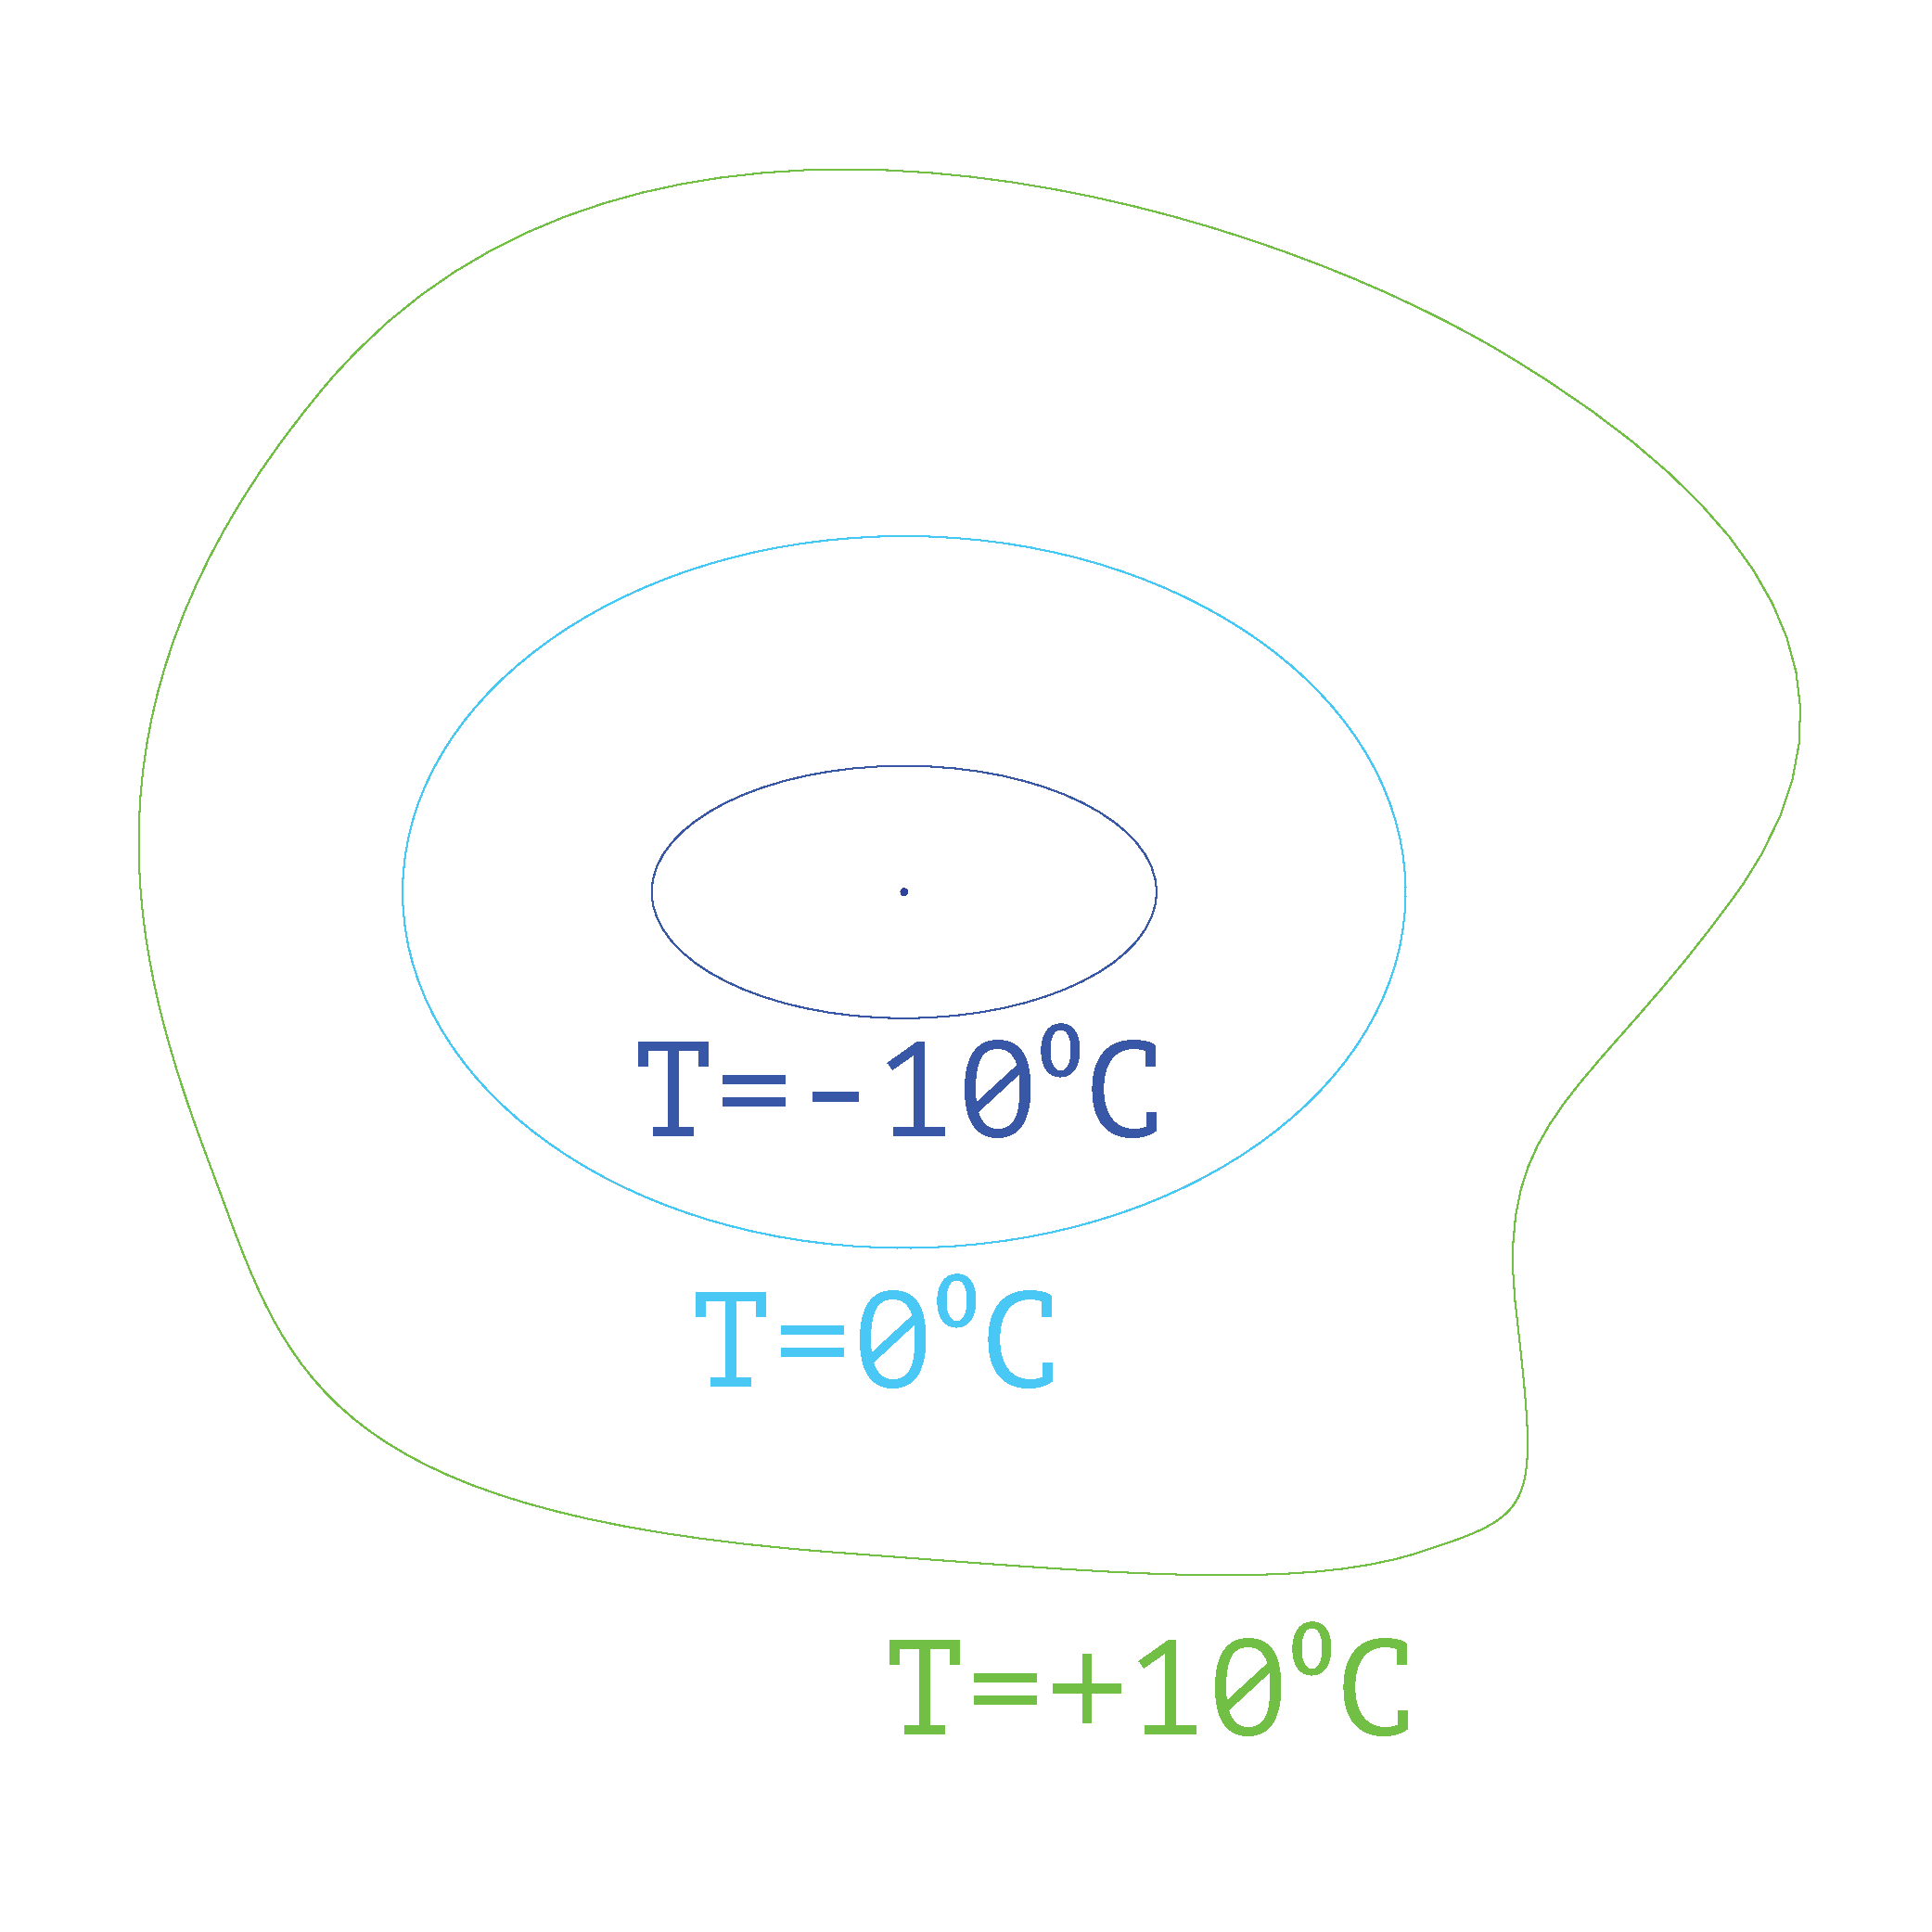
\includegraphics[width=0.47\textwidth]{lec02/temp_lines.pdf} \\ Эквитемпературные линии}
        \end{minipage}
        \hfill
        \begin{minipage}[h]{0.49\textwidth}
        \center{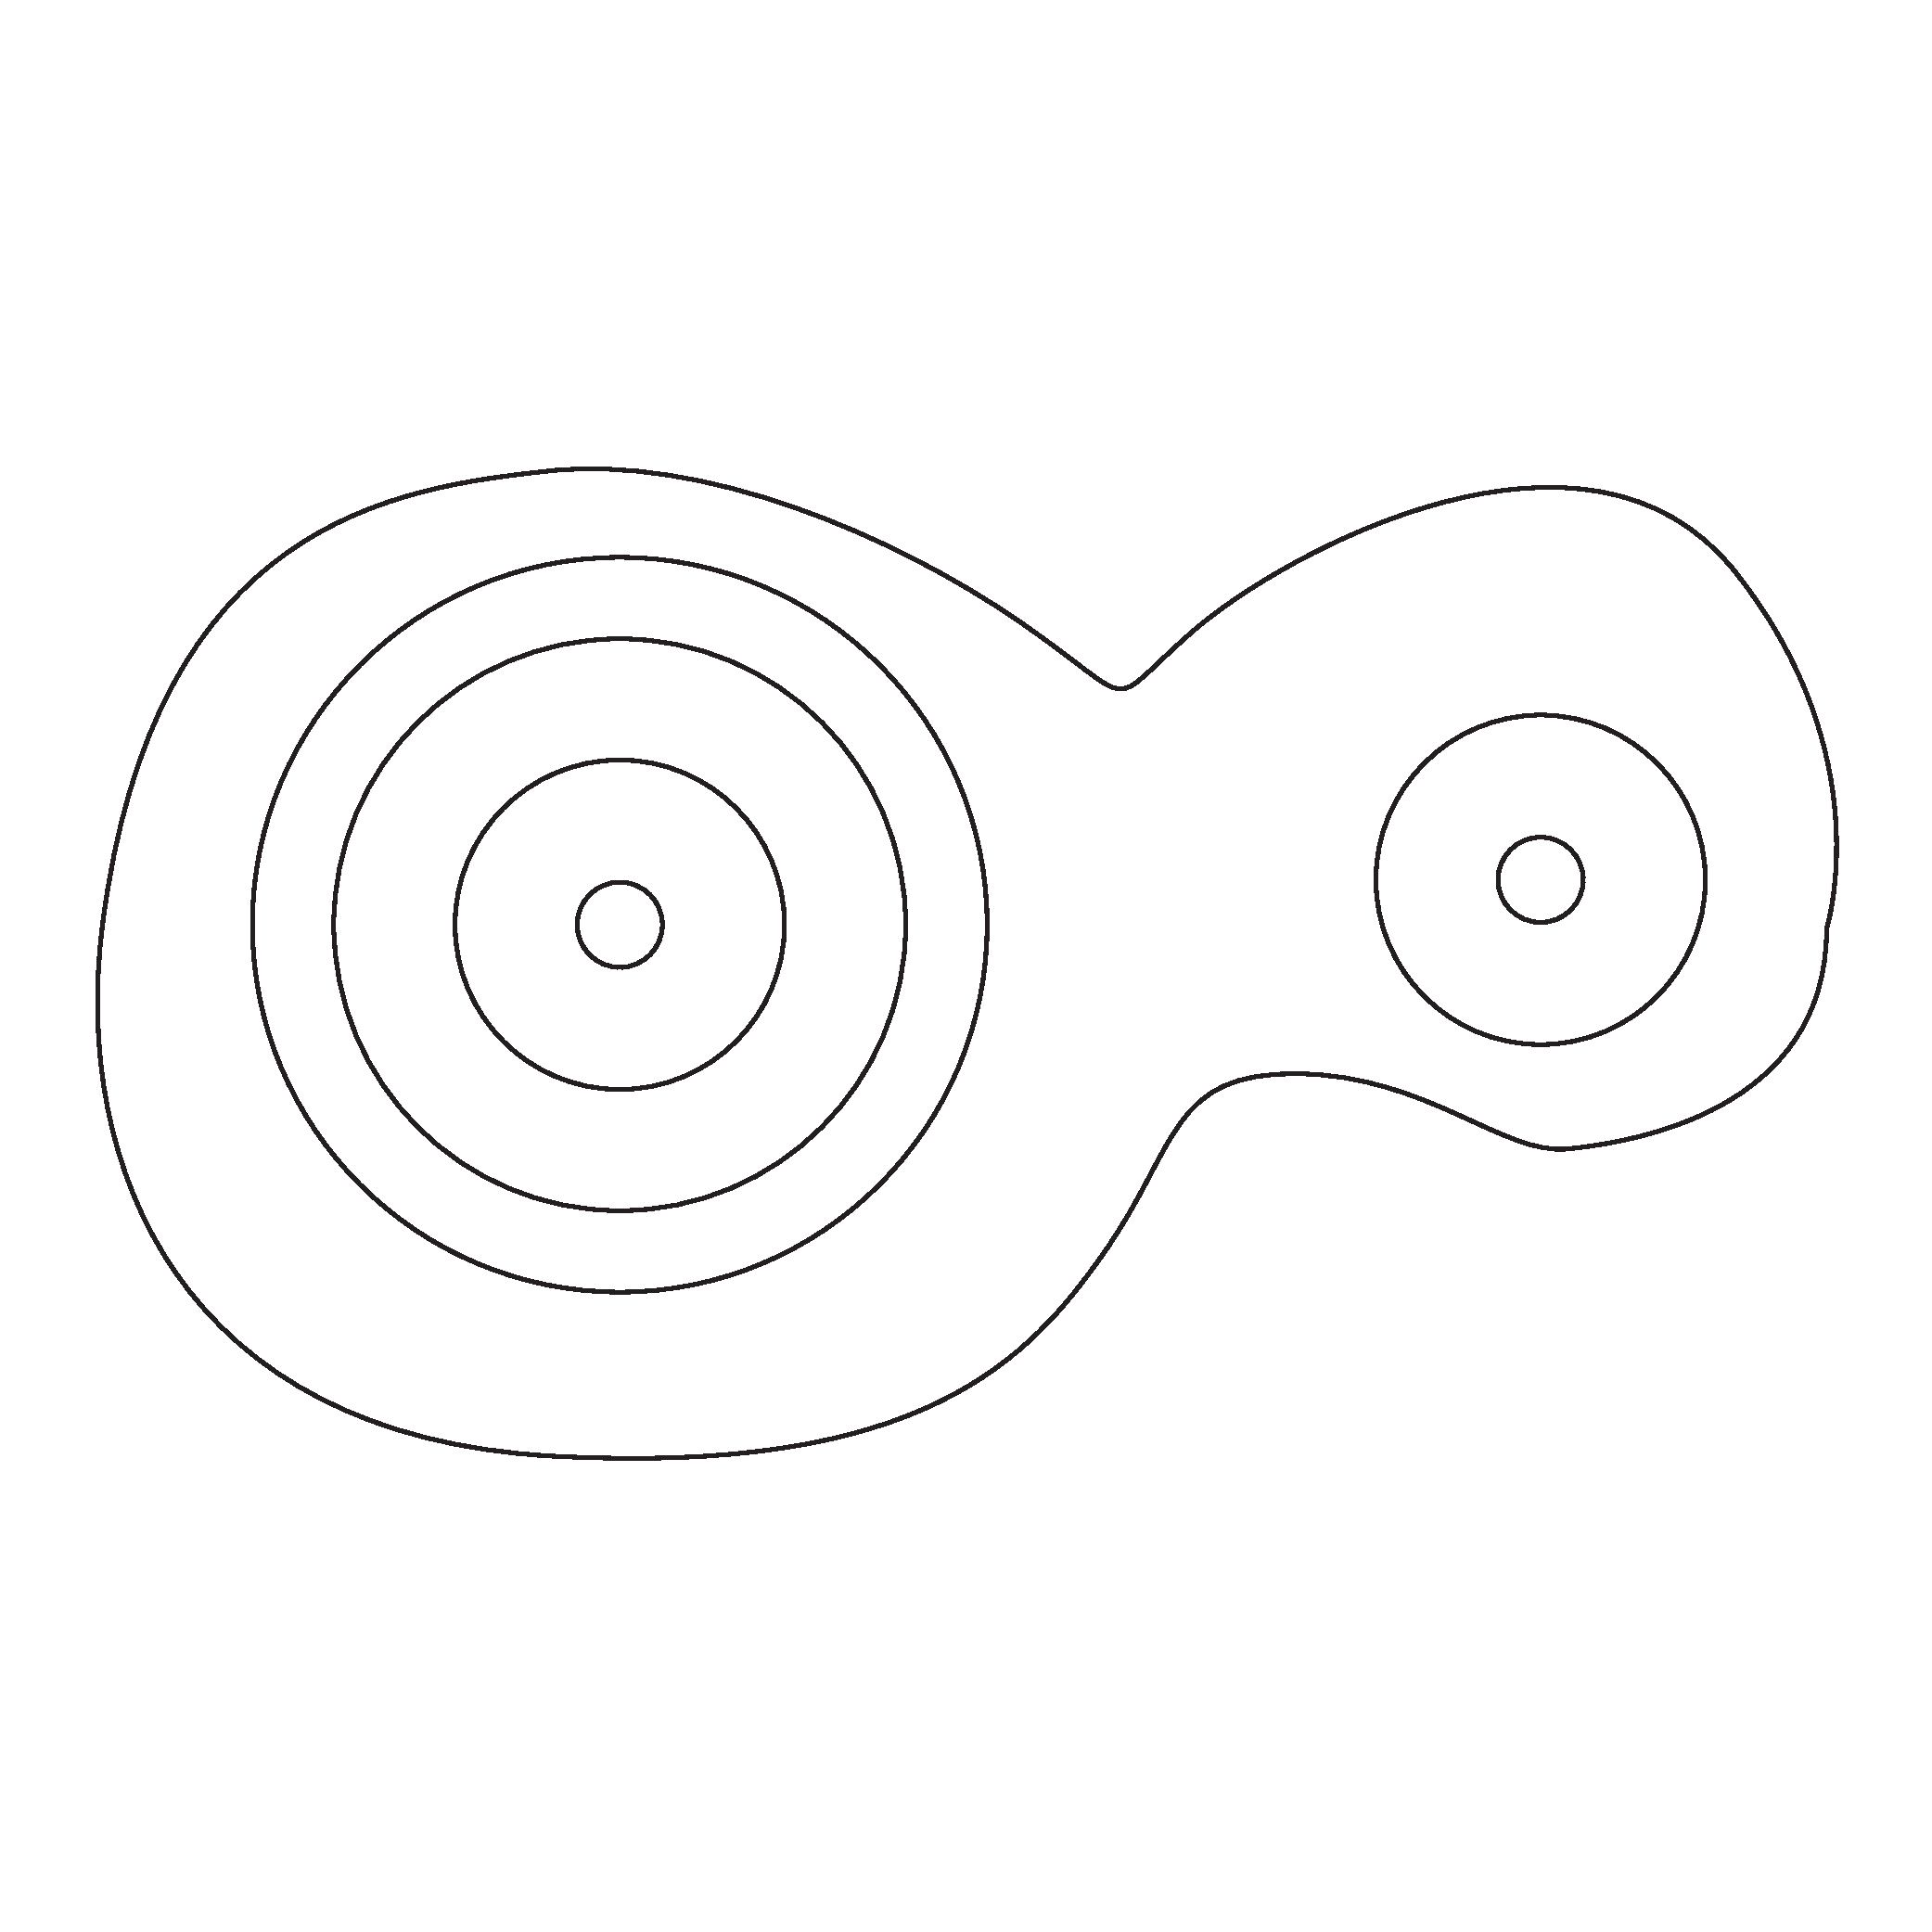
\includegraphics[width=0.47\textwidth]{lec02/height_lines.pdf} \\ Линии равных высот}
        \end{minipage}
    \end{figure}

\subsection{Производная скалярного поля по направлению}

    Пусть задано скалярное поле \( u = u(x,y,z) \). Выберем в нем точку \( M \) и проведём через неё прямую \( l \), задаваемую единичным вектором \( \vec{l} \).

    Составим соотношение:
    \[ \frac{u(M')-u(M)}{MM'}. \]

    Предел этого соотношения
    \[ \lim_{MM'\rightarrow0}\frac{u(M')-u(M)}{MM'} \]
    зависит от направления \( \vec{l} \) -- для \( MM' \) он будет другим в силу \( u(M') = u(M'') \). Этот предел называется производной скалярного поля \( u(x,y,z) \) в точке \( M \) по направлению \( \vec{l} \):
    \[ \der{u}{l} = \frac{u(M')-u(M)}{MM'}. \]
    
    \begin{figure}[h]
        \center
        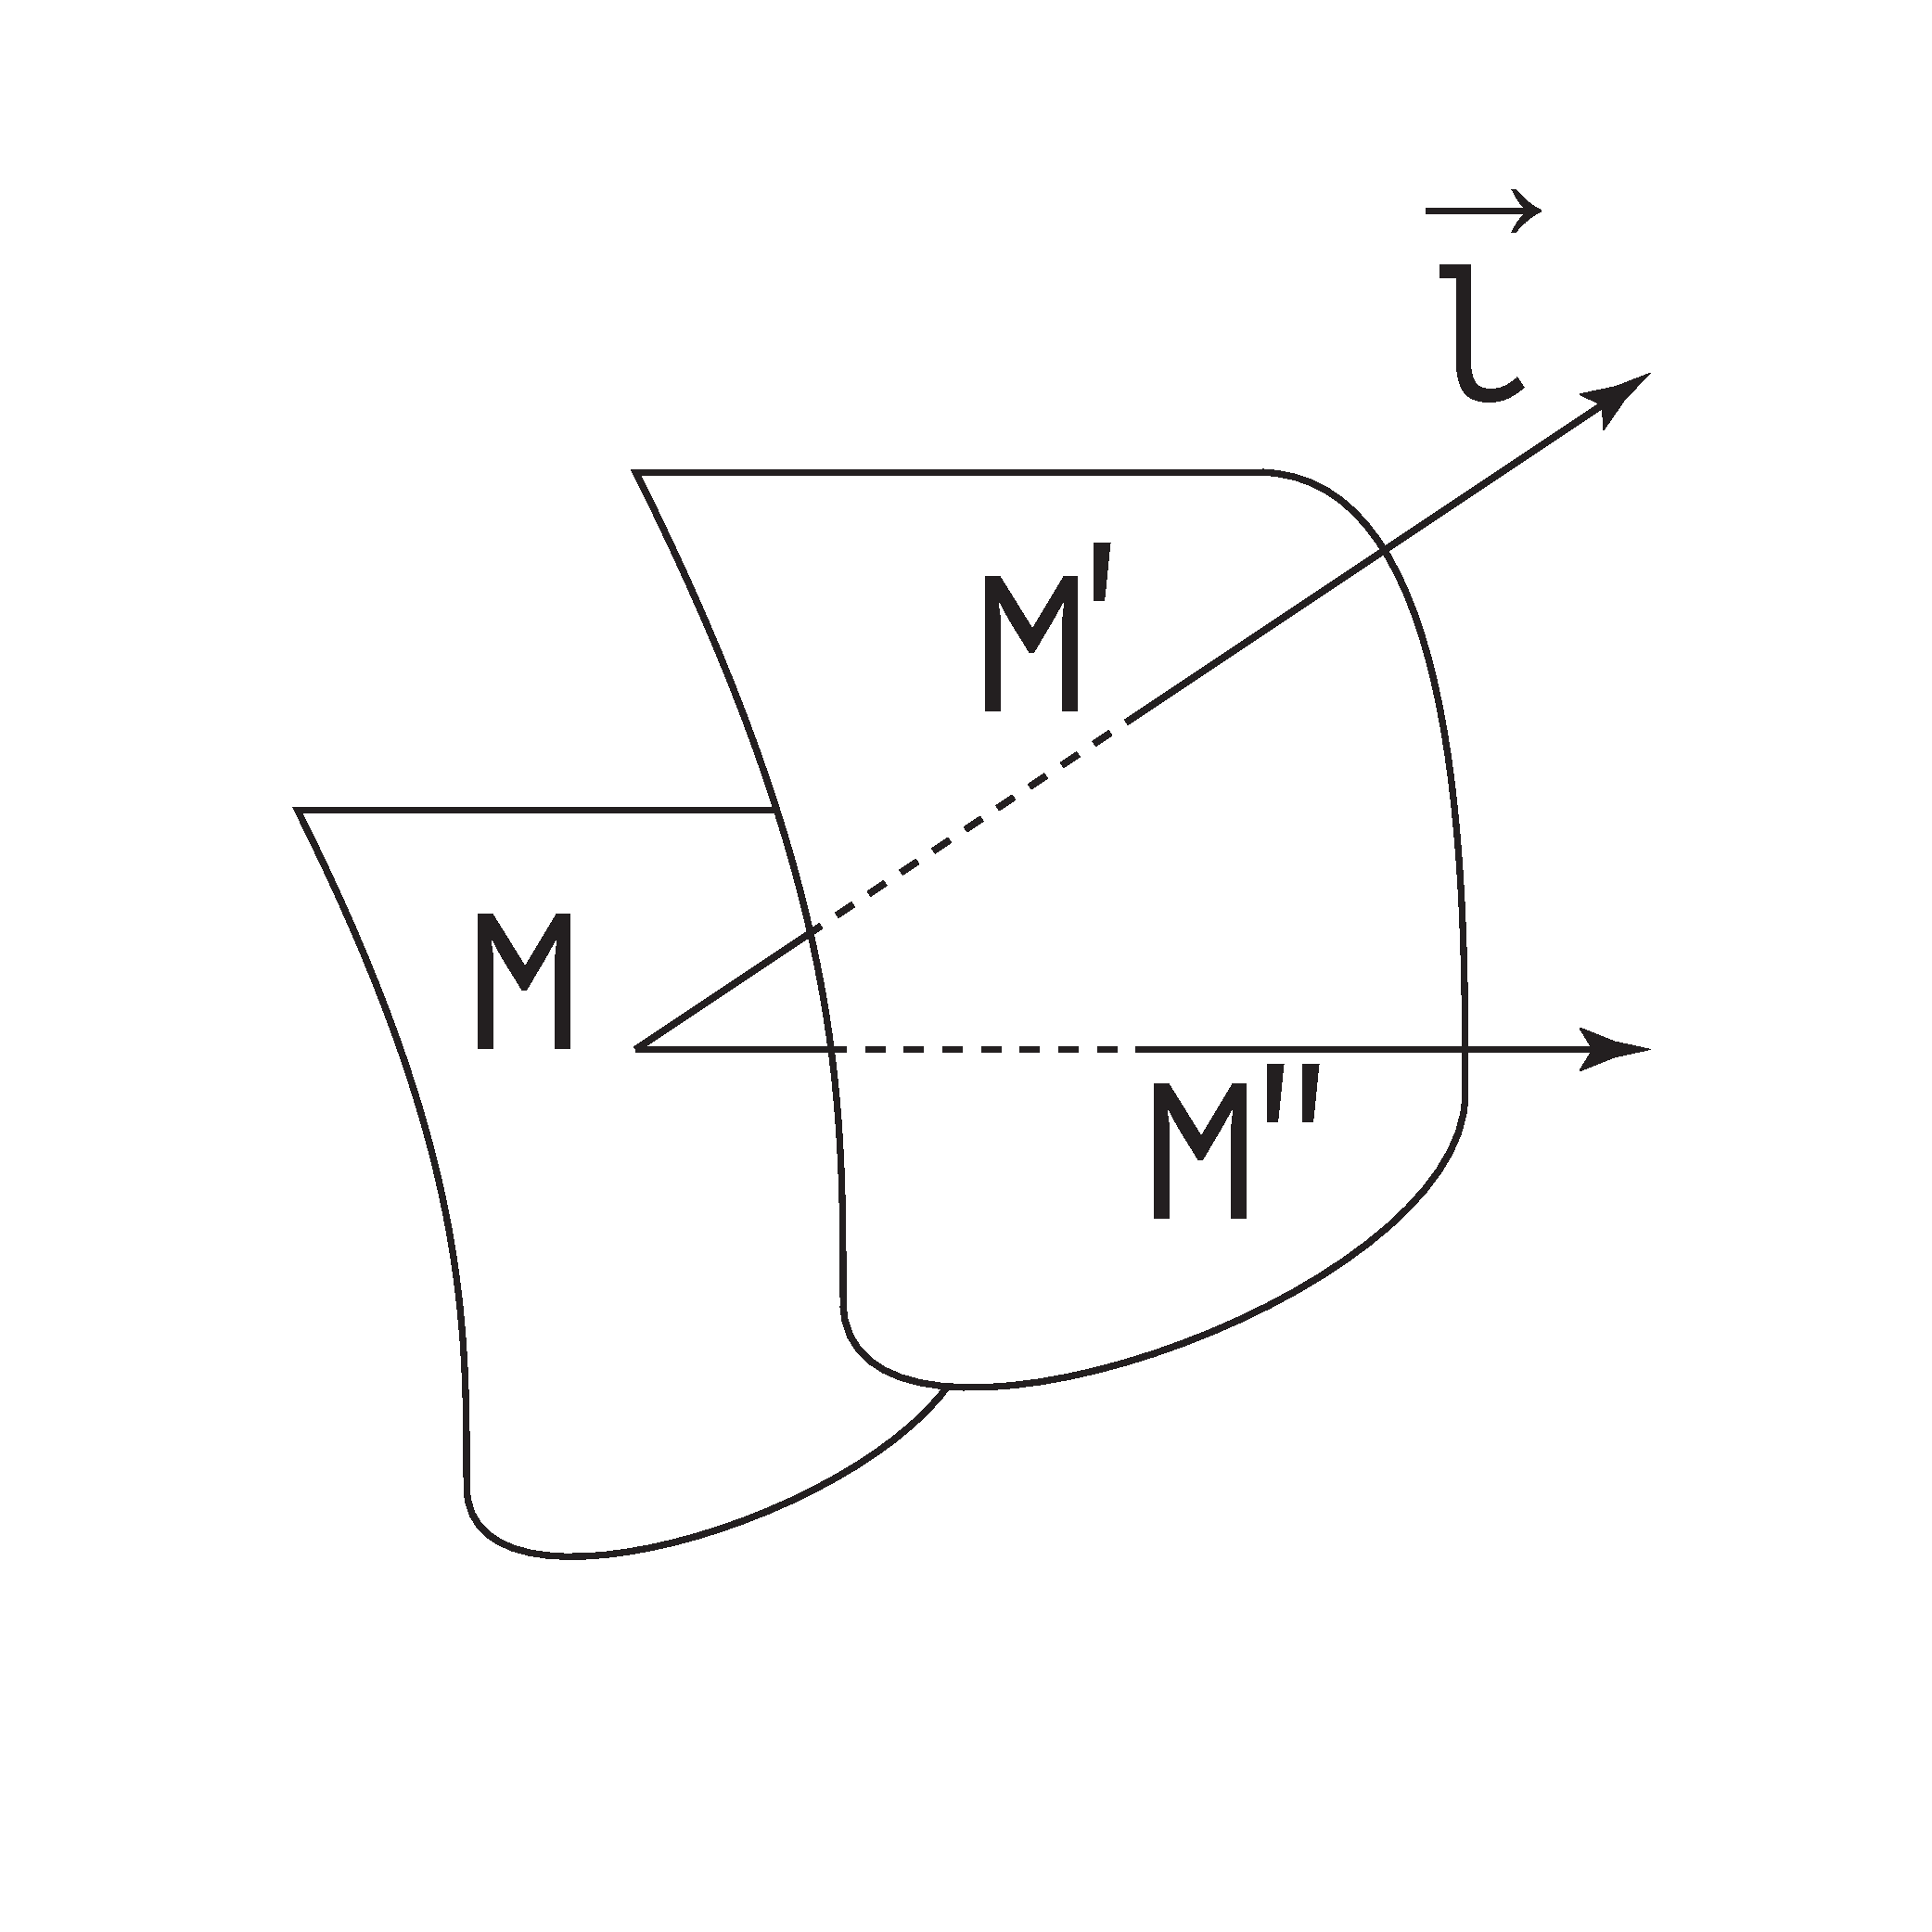
\includegraphics[width=0.47\textwidth]{lec02/derivation_by_direction.pdf}
        \caption{Производная по направлению}
    \end{figure}

    \begin{remark}
        Производная скалярного поля по направлению -- это скаляр.
    \end{remark}

    \begin{remark}
        Производная является инвариантом относительно преобразований базиса.
    \end{remark}

    Чтобы привести выражение для производной к удобной для вычисления форме, запишем его как производную сложной функции:
	\begin{equation}
	\der{u}{l} = \der{u}{x}\cdot\der{x}{l} + \der{u}{y}\cdot\der{y}{l} + \der{u}{z}\cdot\der{z}{l}.
	\label{eq:2.1}
	\end{equation}
    С учётом
    \[ \left\{ \begin{array}{l}
                \der{x}{l} = \frac{l_x}{|\vec{l}|} = l_x = \cos\alpha, \\
                \der{y}{l} = \frac{l_y}{|\vec{l}|} = l_y = \cos\beta, \\
                \der{z}{l} = \frac{l_z}{|\vec{l}|} = l_z = \cos\gamma, \\
            \end{array} \right. \]
    выражение принимает вид:
    \[ \der{u}{l} = \der{u}{x}\cdot\cos\alpha + \der{u}{y}\cdot\cos\beta + \der{u}{z}\cdot\cos\gamma. \]

\subsection{Градиент скалярного поля. Оператор Гамильтона}

    Рассмотрим выражение (\ref{eq:2.1}). Его можно представить как следующее скалярное произведение: \( \vec{l}\cdot\{\frac{\partial u}{\partial x}, \frac{\partial u}{\partial y}, \frac{\partial u}{\partial z}\} \).
    
    Последний вектор называется градиентом скалярного поля \( u(x,y,z) \):
    \begin{equation}
        \gradient u = \left\{\der{u}{x},\ \der{u}{y},\ \der{u}{z}\right\}.
        \label{eq:2.2}
    \end{equation}
    
    Таким образом, выражение (\ref{eq:2.1}) принимает вид:
    \begin{equation}
        \der{u}{l} = \vec{l}\cdot\gradient u.
        \label{eq:2.3}
    \end{equation}
    
    Комбинация производных \( \left\{ \der{}{x},\ \der{}{y},\ \der{}{z}\right\} \) образует символический вектор \( \nabla \) -- оператор дифференцирования, называемый оператором Гамильтона.
    
    Тогда, уравнение (\ref{eq:2.3}) может быть записано в виде:
    \begin{equation}
          \der{u}{l} = \vec{l}\cdot\nabla u. \label{eq:2.4}
    \end{equation}
    
    \begin{remark}
    Уравнение (\ref{eq:2.4}) можно записать в виде
    \begin{equation}
         \der{u}{l} = \left(\vec{l}\cdot\nabla\right)u, \label{eq:2.5}
    \end{equation}
    где \( \vec{l}\cdot\nabla = l_x\der{}{x} + l_y\der{}{y} + l_z\der{}{z} \) -- дифференцирование по направлению.
    \end{remark}
    
    \begin{example}
    Вычислить градиент скалярного поля \( u = \vec{a}\cdot\vec{r} \), где \( \vec{a} = \{ a_x,\ a_y,\ a_z \} = \const \).
    \end{example}    
    
    \begin{solution}
    
    \[ \gradient{u} = \nabla u = \left\{ \der{u}{x},\ \der{u}{y},\ \der{u}{z} \right\} = \{ a_x,\ a_y,\ a_z \} = \vec{a}. \]
    \end{solution}
    
    \begin{example}
    Найти градиент потенциала \( \phi \) поля точечного заряда \( q \): \( \phi = \frac{q}{4\pi\eps_0 r} = k\frac{1}{r} \), где \( r = \sqrt{x^2 + y^2 + z^2} \).
    \end{example}    
    
    \begin{solution}
    
    \[ \nabla\phi = k\nabla\frac{1}{r} = k\{ \der{}{x}\left(\frac{1}{r}\right),\ \der{}{y}\left(\frac{1}{r}\right),\ \der{}{z}\left(\frac{1}{r}\right) \}. \]
    
    Частная производная по \( x \) от \( \frac{1}{r} \):
    \[ \der{}{x}\left(\frac{1}{r}\right) = -\frac{1}{r^2}\cdot\der{r}{x} = -\frac{x}{r^3}. \]
    
    Аналогично, производные по \( y \) и \( z \):
    \[ \begin{array}{l}
	\der{}{y}\left(\frac{1}{r}\right) = -\frac{y}{r^3}; \\
	\der{}{z}\left(\frac{1}{r}\right) = -\frac{z}{r^3}.
    \end{array} \]
    
    Окончательно,
    \[ \nabla\varphi = -k\frac{1}{r^3}\{ x, y, z \} = -k\frac{\vec{r}}{r^3} = -\frac{q\vec{r}}{4\pi\eps_0 r^3} = -\vec{E} \text{ -- электрическое поле} \]
    \end{solution}
% subsection Градиент скалярного поля. Оператор Гамильтона (end)

	\subsection{Свойства градиента}
	\begin{enumerate}
	\item Вектор \( \gradient{u} \) перпендикулярен поверхности уровня \( u(x, y, z) = \const \) в любой его точке.	
	\begin{proof}
	
	Рассмотрим поверхность уровня \( u(x, y, z) =\const \). Пусть \( \vec{l}_\mathrm{\tau} \) касательный единичный вектор к ней в точке \( M \). А так как, по определению поверхности уровня, \( u = \const \), то \( \der{u}{l_\mathrm{\tau}} = \vec{l}_\mathrm{\tau}\cdot\nabla u = 0 \). Следовательно, \( \nabla u \perp \vec{l}_\mathrm{\tau} \) для любого касательного вектора и поверхности уровня в точке \( M \).
	\end{proof}
	
	\item Функция \( u(x, y, z) \) растет вдоль направления \( \nabla u \).
	\begin{proof}
	
	Вычислим производную по направлению градиента \( \nabla u \):
	\[ \der{u}{l} = \vec{l}\cdot\nabla u = |\vec{l}|\cdot|\nabla u| > 0, \]
	следовательно, функция возрастает вдоль направления градиента.
	\end{proof}
	
	\item Скорость роста поля \( u \) масимальна вдоль направления градиента.
	\begin{proof}
	
	\[ \der{u}{l} = \vec{l}\cdot\nabla u = |\vec{l}|\cdot|\nabla u|\cos\alpha. \]
	Это произведение максимально при \( \alpha = 0 \), то есть при \( \vec{l} \uparrow\uparrow \nabla u \).
	\end{proof}
	\begin{corollary}
	Пусть \( \vec{n} \) -- единичный вектор нормали к поверхности уровня \( u(x, y, z) = \const \). Тогда производная по направлению нормали:
	\[ \der{u}{n} = |\nabla u|\cdot|\vec{n}|\cos0 = |\nabla u|. \]
	\end{corollary}
	\begin{corollary}
	Единичный вектор нормали \( \vec{n} \) может быть представлен в виде
	\[ \vec{n} = \frac{\nabla u}{|\nabla u|}. \]
	\end{corollary}
	
	\item Пусть \( \vec{a} \) и \( \vec{b} \) -- два скалярных поля, тогда:
	\begin{enumerate}
	\item \( \nabla(u + v) = \nabla u + \nabla v; \)
	\item \( \nabla(uv) = u\nabla v + v\nabla u. \)
	\end{enumerate}
	\begin{proof}
	
	\begin{enumerate}
	\item \( \nabla(u + v) = \left\{ \der{(u + v)}{x},\der{(u + v)}{y}, \der{(u + v)}{z} \right\} = \nabla u + \nabla v. \)
	\item \( \nabla(uv) = \left\{ \der{uv}{x}, \der{uv}{y}, \der{uv}{z} \right\} = u\nabla v + v\nabla u. \)
	\end{enumerate}
	\end{proof}
	\end{enumerate}

	\begin{example}
	Найти нормаль поверхности уровня скалярного поля \( u = x^2 + y^2 \) в точке \( M(3, 4) \).
	\end{example}
	\begin{solution}
	
	Градиент поля:
	\[ \nabla u = \{ 2x, 2y \}. \]
	
	Нормаль:
	\[ \vec{n} = \frac{\nabla u_n}{|\nabla u_n|} = \frac{\{ 6, 8 \}}{10} = \{ 0.6, 0.8 \}. \]
	
	\begin{remark}
	Линии поля \( u = x^2 + y^2 \) -- концентрические окружности.
	\end{remark}
	
	\begin{remark}
	Если поле \( u \) плоское, то есть \( u = u(x, y) \), то вектор градиента перпендикулярен линии уровня в данной точке.
	\end{remark}
	\end{solution}
	
	\begin{example}
	Вычислить производную скалярного поля \( u = \frac{x}{y} - \frac{y}{x} \) в точке \( M(1, 1) \) по направлению к точке \( M’(4, 5) \).
	\end{example}
	\begin{solution}
	
	Направляющий вектор:
	\[ \vec{l} = \left\{ \frac{3}{5}, \frac{4}{5} \right\}. \]
	
	Градиент поля в точке \( M \):
	\[ \gradient{u}_M = \left\{ \left.\der{u}{x}\right|_M, \left.\der{u}{y}\right|_M \right\} = \left\{ \frac{1}{y} + \frac{y}{x^2}, -\left(\frac{x}{y^2} + \frac{1}{x}\right) \right\} = \{ 2, -2 \}. \]
	
	Производная по направлению:
	\[ \left.\der{u}{l}\right|_M = 2\cdot\frac{3}{5} - 2\cdot\frac{4}{5} = -\frac{2}{5}. \]
	\end{solution}
	
	\begin{appendix} Поверхности второго порядка:
	
	Общее уравнение:
	\[ \sum\limits_i \sum\limits_j a_{ij}x_ix_j + \sum\limits_i b_ix_i + c = 0. \]
	
	Канонические уравнения:
	\begin{enumerate}
	\item Эллипсоид:
	\[ \frac{x^2}{a^2} + \frac{y^2}{b^2} + \frac{z^2}{c^2} = 1. \]
	
	\item Однополостный гиперболоид:
	\[ \frac{x^2}{a^2} + \frac{y^2}{b^2} - \frac{z^2}{c^2} = 1. \]
	
	\item Двухполостный гиперболоид:
	\[ \frac{x^2}{a^2} + \frac{y^2}{b^2} - \frac{z^2}{c^2} = -1. \]
	
	\item Конус:
	\[ \frac{x^2}{a^2} + \frac{y^2}{b^2} - \frac{z^2}{c^2} = 0. \]
	
	\item Эллиптический параболоид:
	\[ \frac{x^2}{a^2} + \frac{y^2}{b^2} = z. \]
	
	\item Гиперболический параболоид:
	\[ \frac{x^2}{a^2} - \frac{y^2}{b^2} = z, \]
	при повороте на \( \frac{\pi}{4} \) получим:
	\[ xy = Cz. \]
	
	\item Параболический цилиндр:
	\[ y = ax^2. \]
	
	\item Гиперболический цилиндр:
	\[ \frac{x^2}{a^2} - \frac{y^2}{b^2} = 1. \]
	
	\item Параболический цилиндр:
	\[ \frac{x^2}{a^2} + \frac{y^2}{b^2} = 1. \]
	
	\item Пара плоскостей:
	\[ \frac{x^2}{a^2} - \frac{y^2}{b^2} = 0; y = \pm kx. \]
	\end{enumerate}
	\end{appendix}
